\section{Implementation} \label{implementation}
Below are the different components which have been implemented to support this research. The entire implementation exists inside the Breda repository and is written in rust and HLSL, this is why all code samples also use these langauges.

\begin{wrapfigure}{r}{0.5\textwidth}
    \centering
    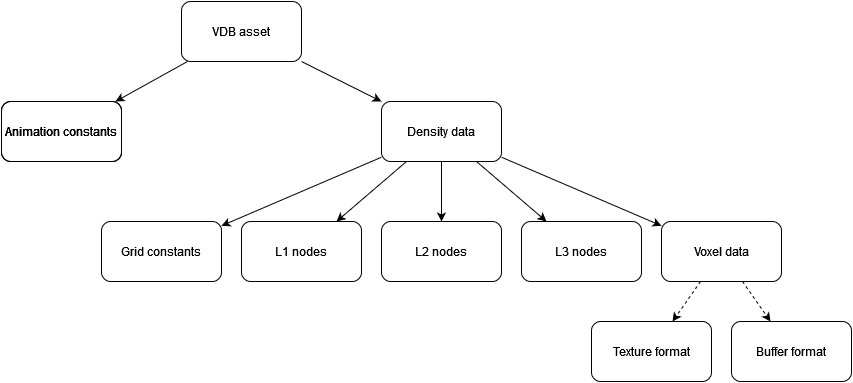
\includegraphics[width=\linewidth]{figures/vdb_asset.png}
    \caption{VDB asset data structure. Each VDB asset has constants for the entire animation, and density data. This density data has all the constants, nodes and voxel data. This voxel data can either be in buffer or texture format. }
    \label{fig:vdb_asset}
\end{wrapfigure}

\subsection{Asset pipeline} \label{implementation:asset_pipeline}
The Breda asset pipeline is used to load all VDB files. This allows us to specify how our assets are loaded and processed, along with caching our final assets to reduce the amount of rebuilding. The main tweakable options for our VDB asset processing pipeline are the format, grid, filenames and clustering options. Format can be any of 32bit floating point, 16bit floating point, unsigned normalized (8bit float between 0 and 1) and BC7 \ref{introduction:texture_compression}. The grid specifies which grid in the VDB file we use as our density data. Usually there are multiple grids in each VDB file, we can have density, temperature and volume type for example. All of these grids are used for different parts in a rendering pipeline, but for this research we are only interested in a single grid and that is the density grid. The filenames option is used to select one or multiple VDB files, when entering multiple filenames we assume that these are an animation sequence. The clustering options consist of three things: (1) number of clusters, which is $k$ when running k-means. (2) The number of iterations of k-means. And (3) the variance rejection threshold, which is used to specify how heterogeneous our bricks can be before we stop clustering them.

Using these options we can compute our VDB asset. This consists mostly of constants and GPU-friendly vectors of data (see Figure \ref{fig:vdb_asset}). All nodes are implemented as structs which contain an unsigned integer to point into the next level of nodes, and an array which contains unsigned integers. These are interpreted as the active child bitmasks. In code we refer to the internal nodes as L1, L2 and L3 nodes. L1 being the top level node with size $(1 << 5)^3$, L2 having size $(1 << 4)^3$ and L3 having size $(1 << 3)^3$ and pointing into the voxel data. The diffferent animation frames are all unique L1 nodes. So if we want to render a specific frame we can simply take the frame id and use that to index into the L1 nodes buffer, all pointers after that are handled at the asset creation stage.

The actual asset creation process has a few steps. First we read the metadata of our VDB files. We then use these to select which grid we want to read, after which we load the VDB data using vdb-rs \cite{VDBRS} which was developed during this research. Then we transform this data into our flat GPU friendly data. After which we perform our post processing transformations. We first run our deduplication scheme described in Section \ref{approach:clustering_similar_nodes}. After this we transform our data format from our easy (and locally coherent) buffer format, to the texture format. Then, depending on which format options were used, we compress our data. So we reduce our floating point data to either 16bit, 8bit or Bc7 texture data. After which we upload everything to the GPU.


\subsection{Shaders} \label{implementation:shaders}
\subsection{Texture formats} \label{implementation:texture_formats}
\subsection{Libraries} \label{implementation:libraries}



\subsection{VDB viewer} \label{implementation:vdb_viewer}
A prototyping application was created for visualizing VDB files. This application can be used to load a single VDB file and display multiple debug views of the model as can be seen in Figure \ref{implementation:vdb_viewer:debug_views}.

\begin{figure}[H]
    \centering
    \subfloat[Shaded by accumulating density along primary ray. The body of the cloud is hollow as can be seen.]{
        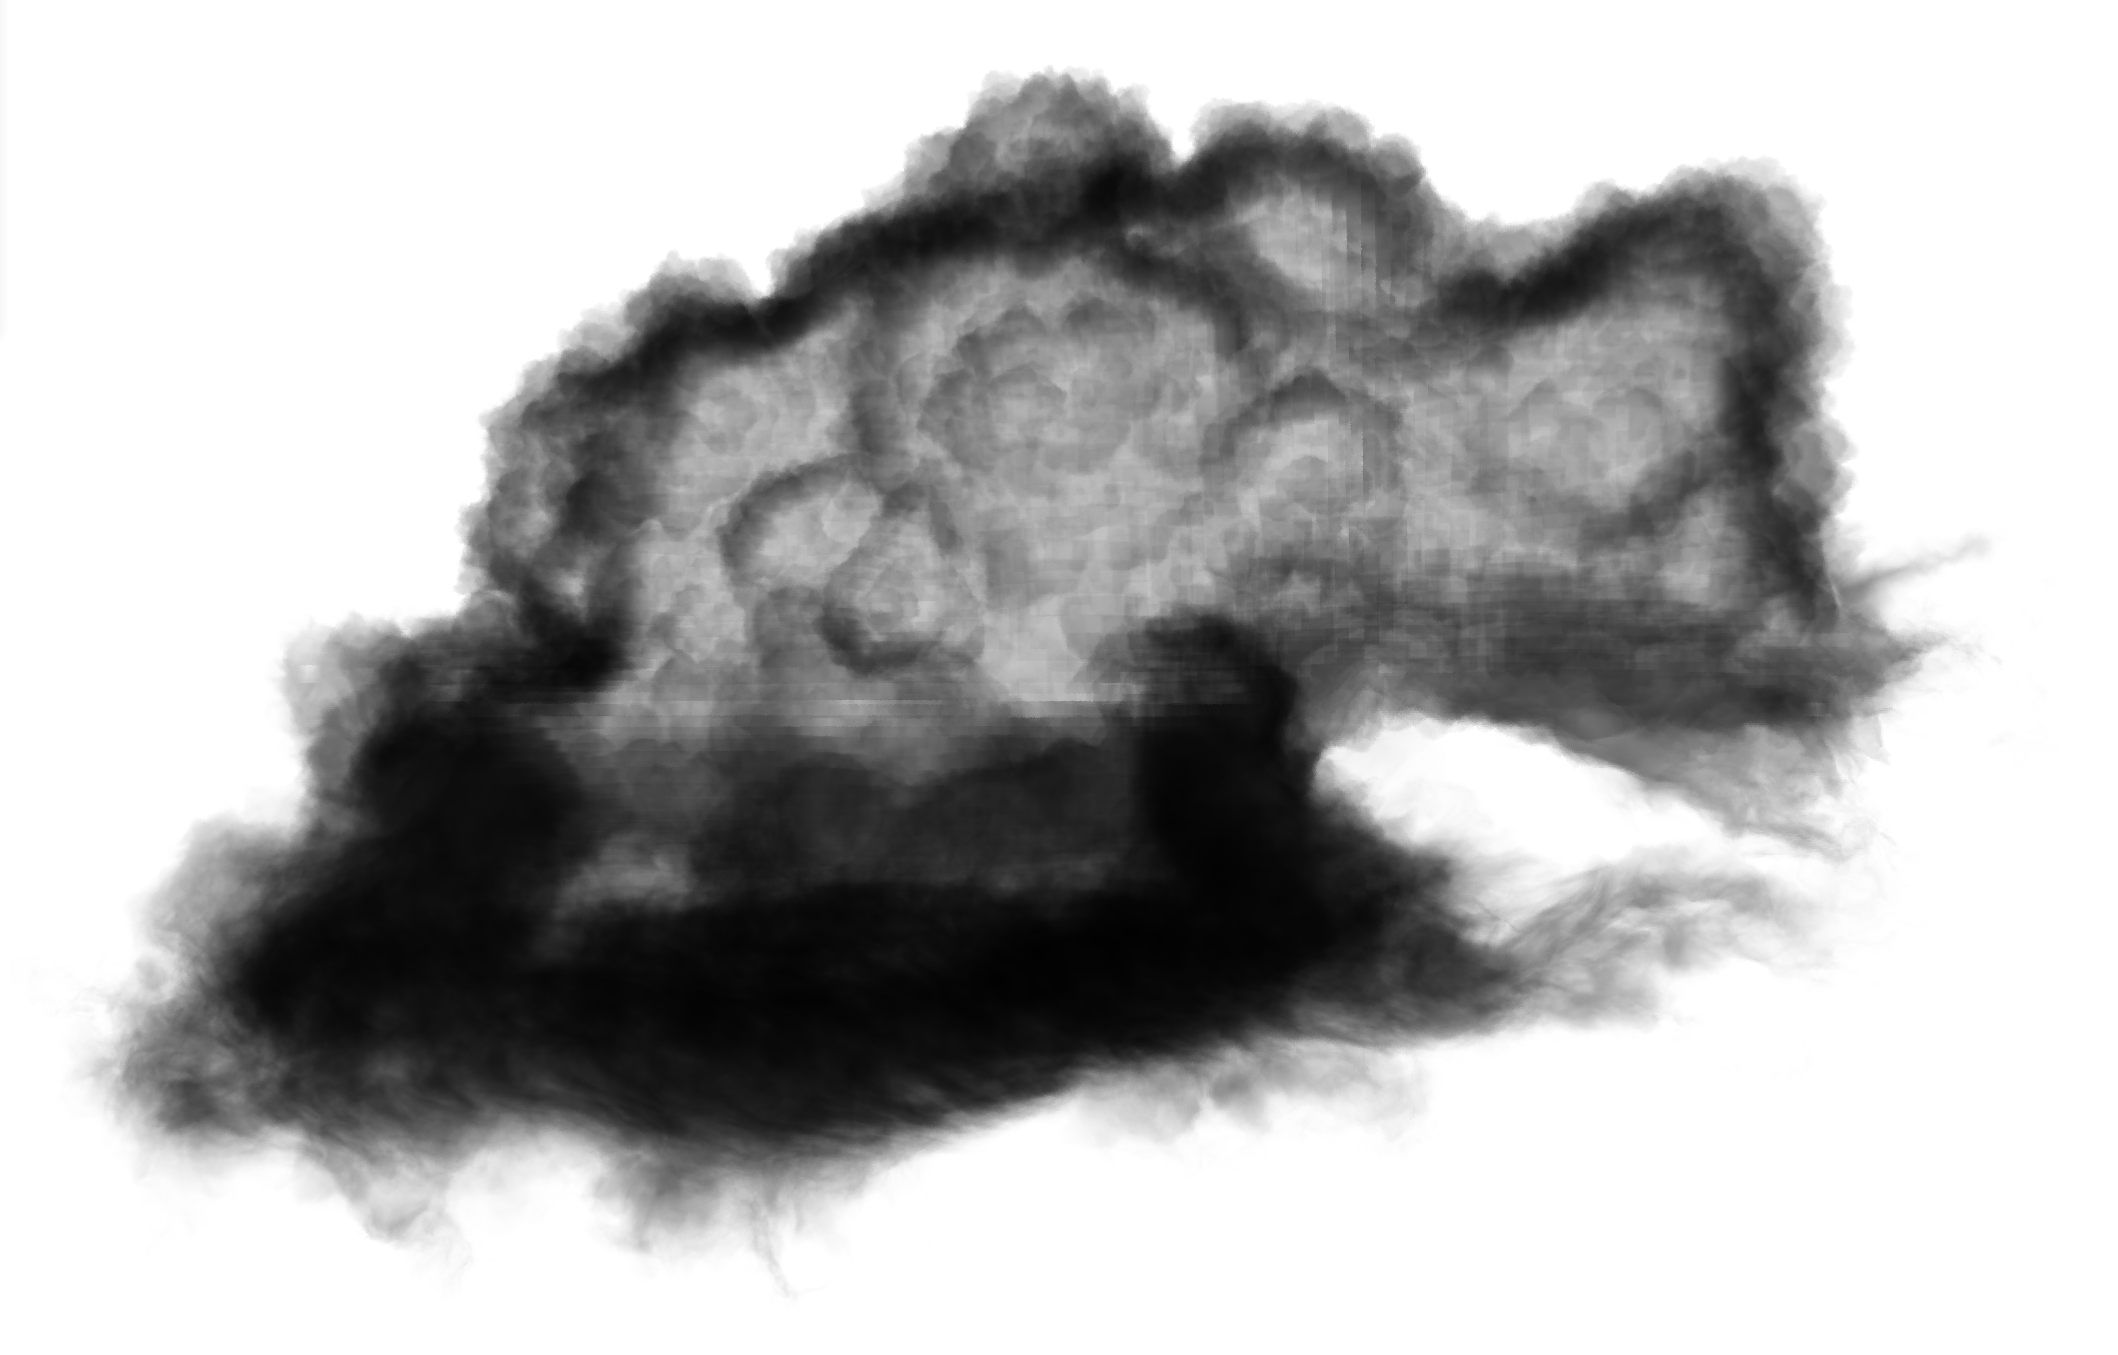
\includegraphics[width=0.45\textwidth]{figures/disney_cloud_half_res_shaded.png}
    }
    \hfill
    \subfloat[Shaded by depth of first hit voxel.]{
        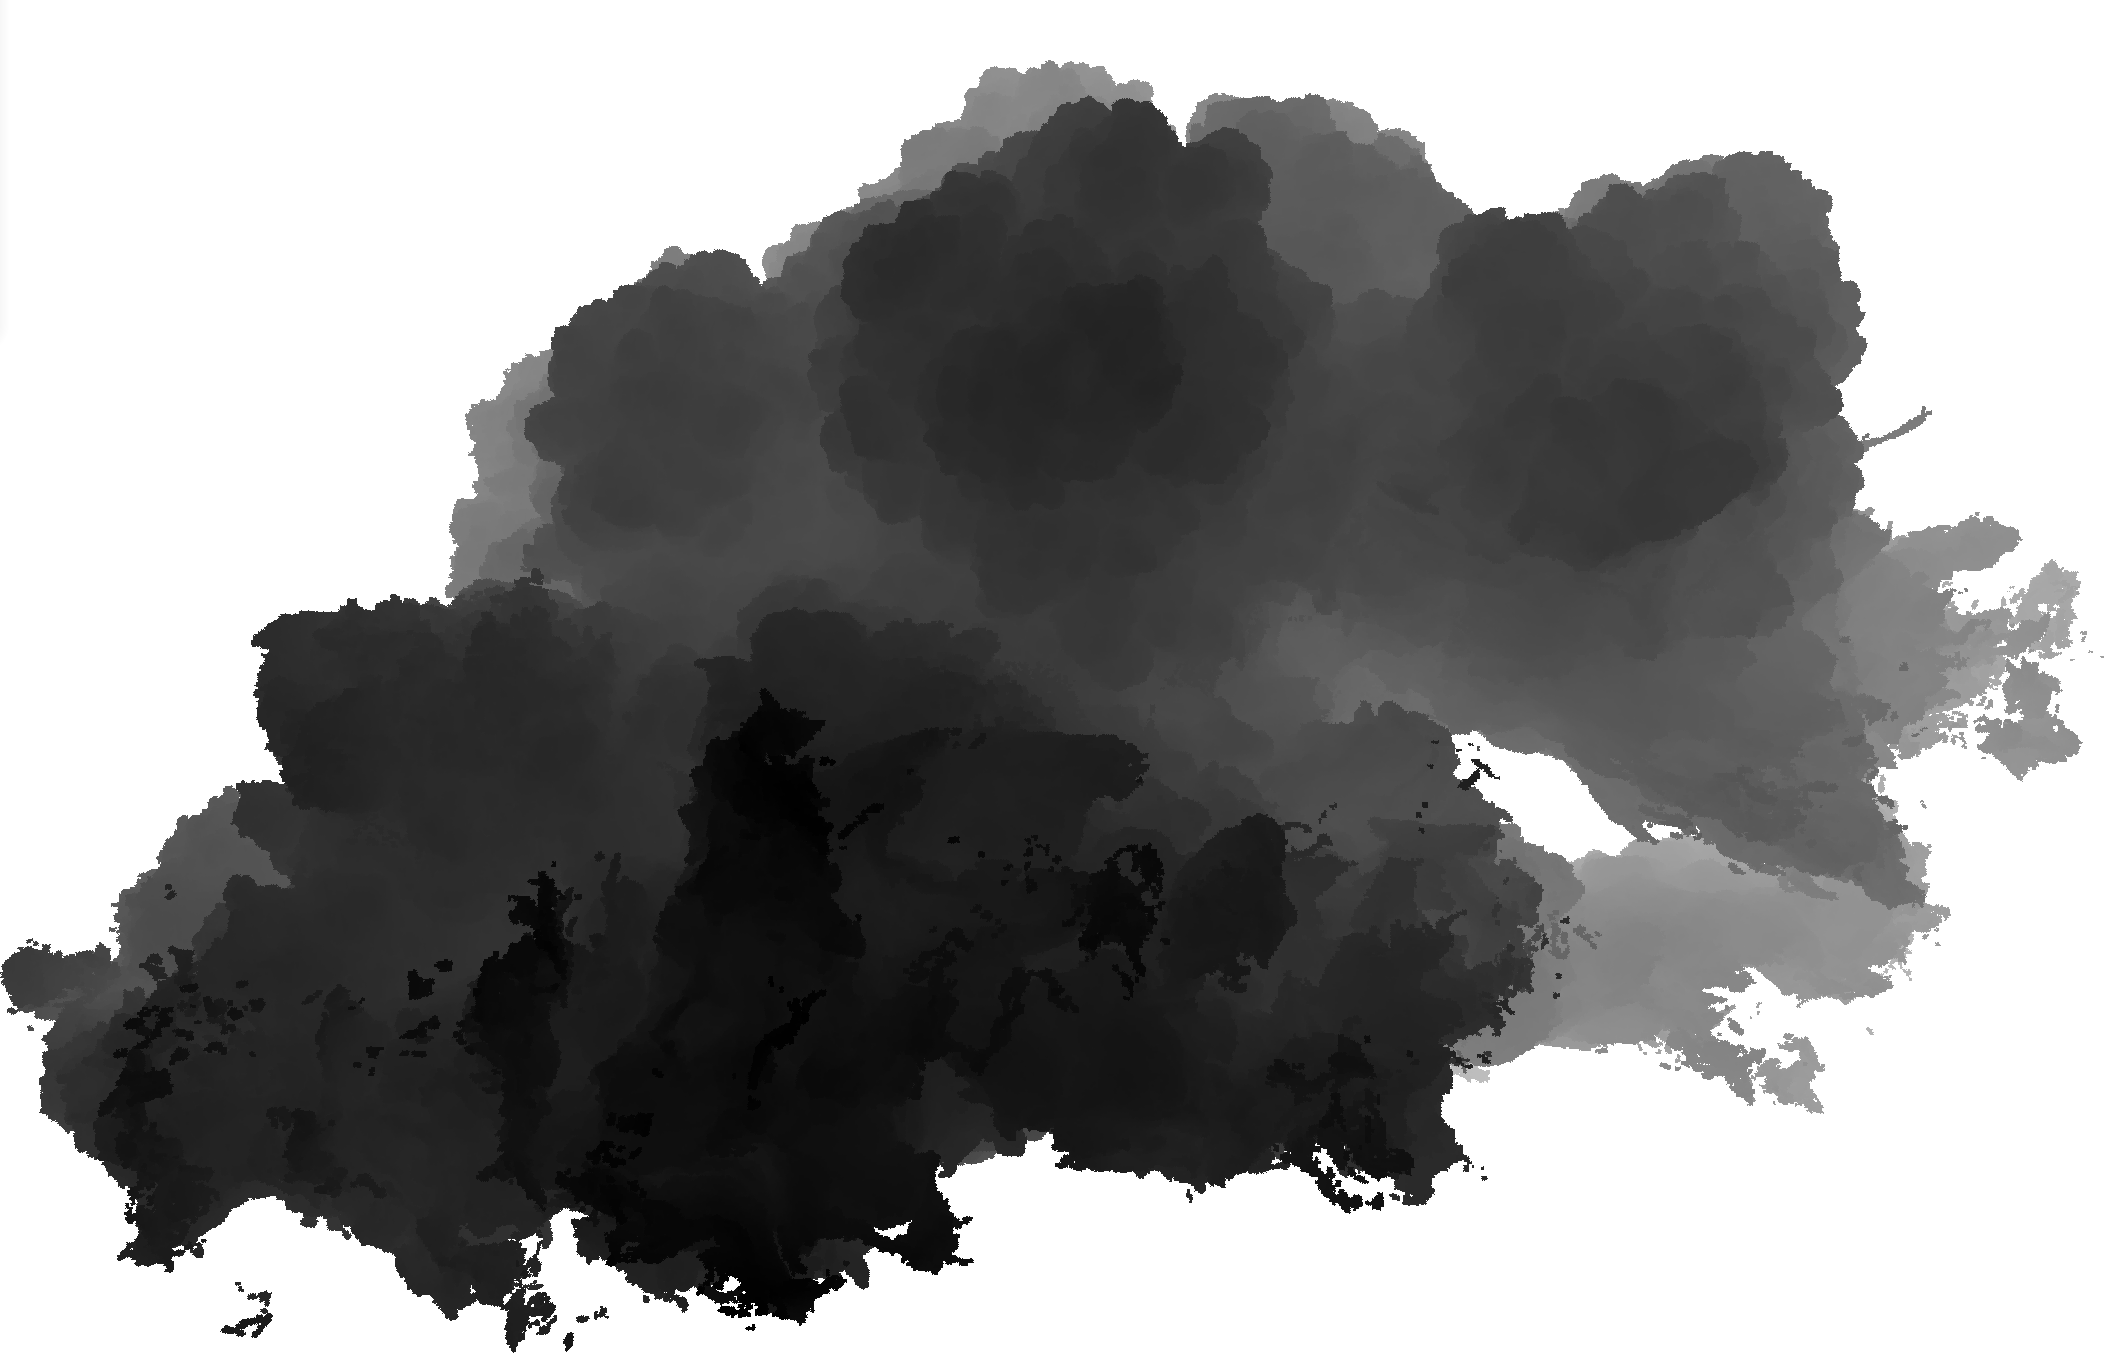
\includegraphics[width=0.45\textwidth]{figures/disney_cloud_half_res_depth.png}
    }
    \hfill
    \subfloat[Shaded by index into the voxel index. Shown is a conversion from index to hue using the following formula: $x + y\times dim\_size + z\times dim\_size^2$. The striped pattern is a result of bricks ($8^3$ voxels) are a combination two texture slices, these are the altering index colors. The larger shifts in color, which are in very specific cubic regions, correlate to the different level 2 internal nodes.]{
        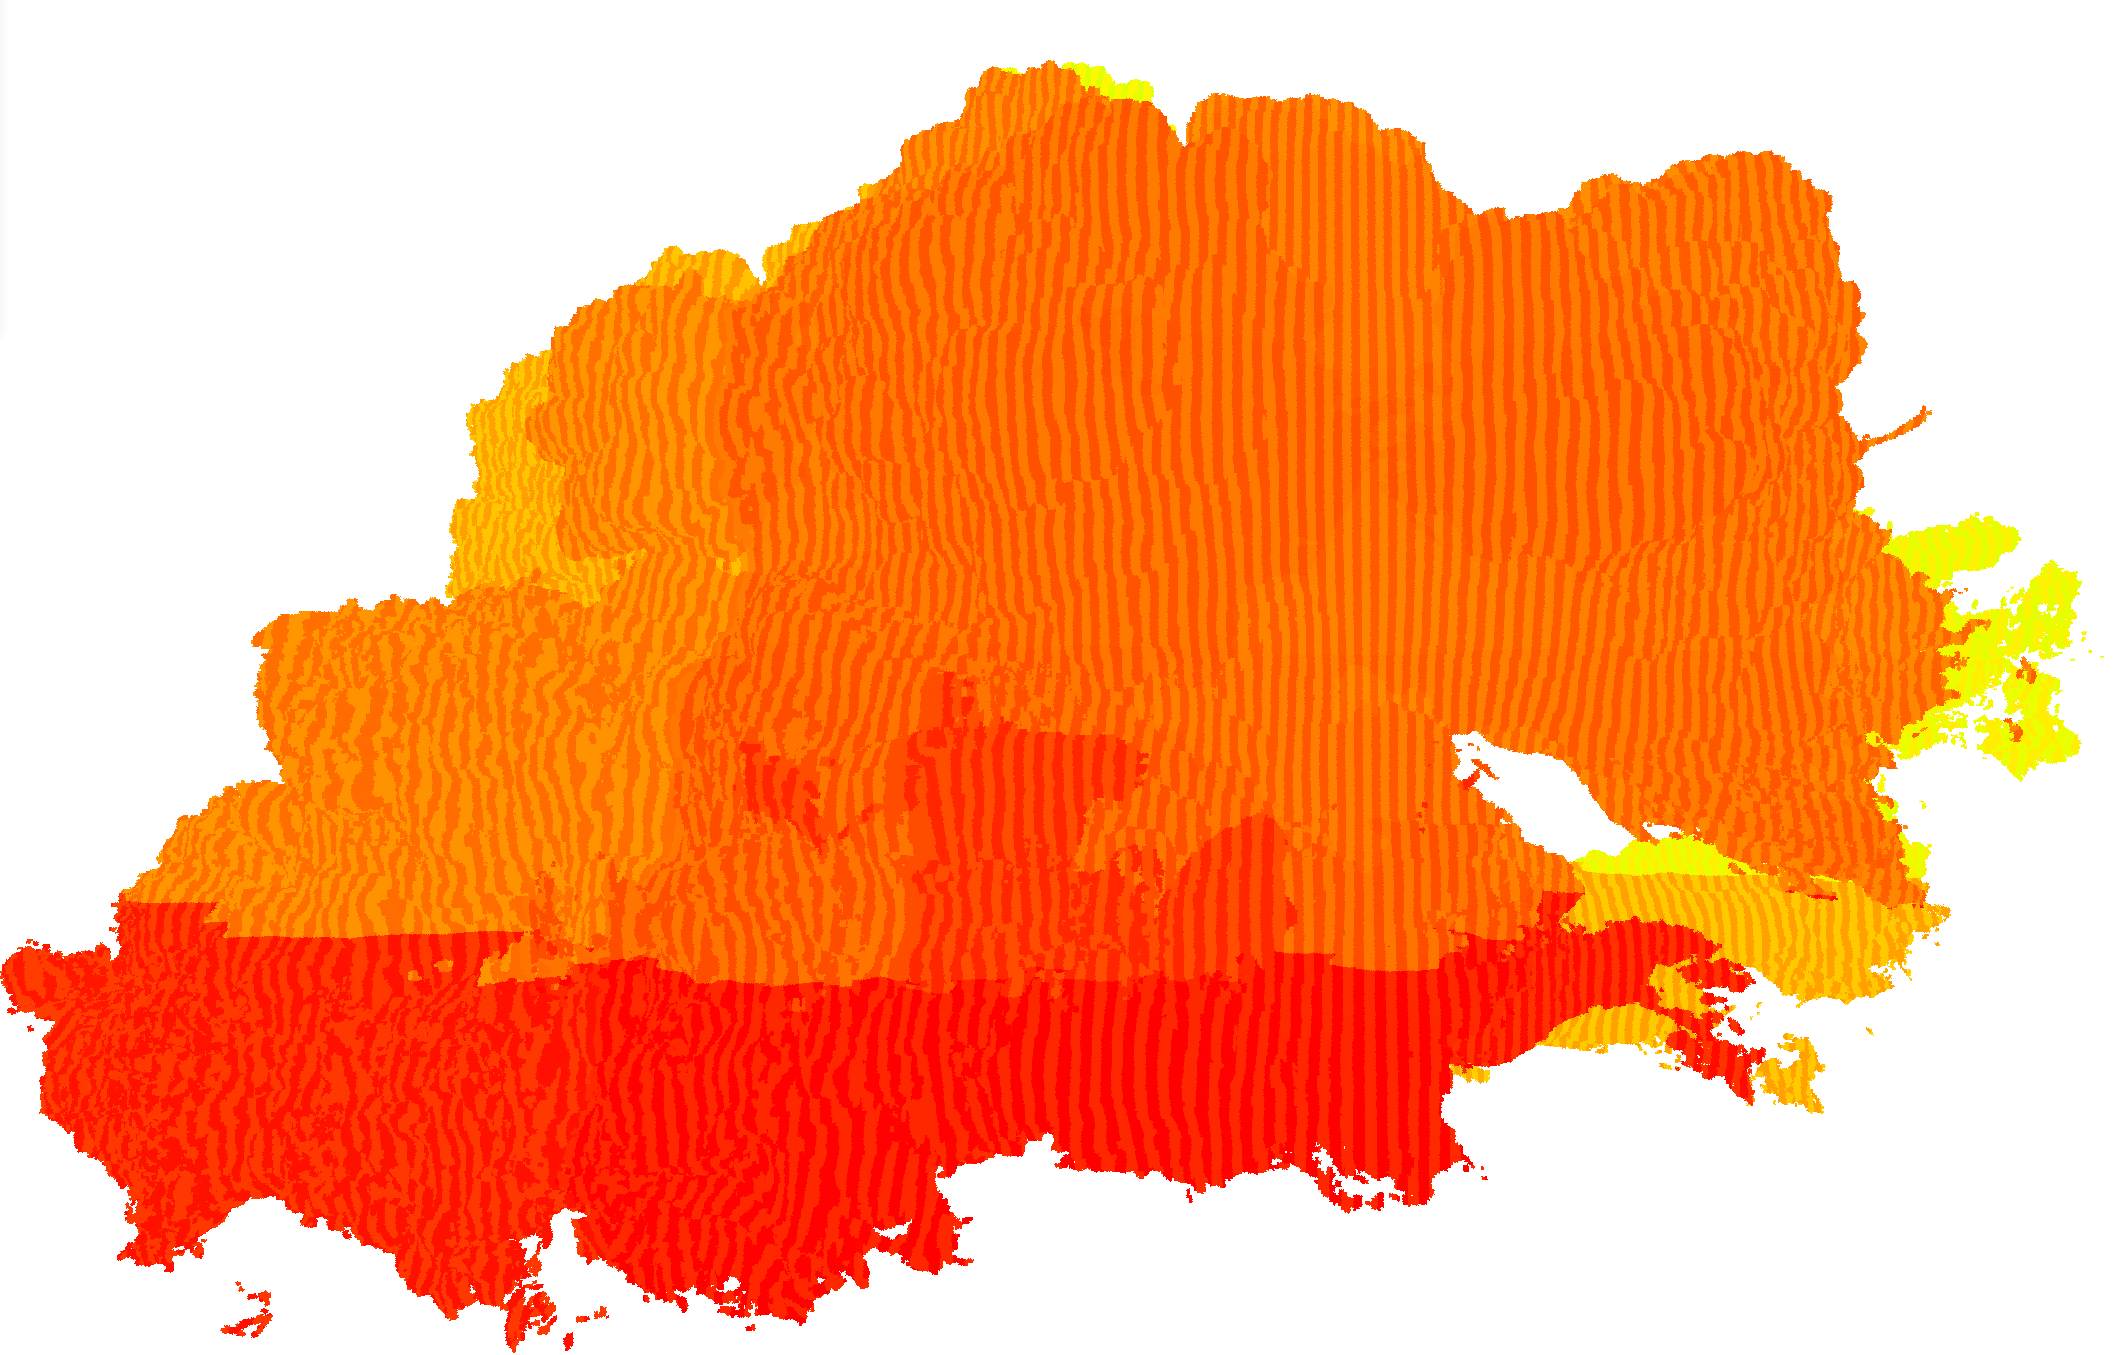
\includegraphics[width=0.45\textwidth]{figures/disney_cloud_half_res_index.png}
    }
    \hfill
    \subfloat[Shaded by density of first hit voxel, where a low density is red and a high density results in different hue's. Overall the entire outside of the cloud only shows low density voxels, but there are some spots where deeper voxels are visible which have a higher density.]{
        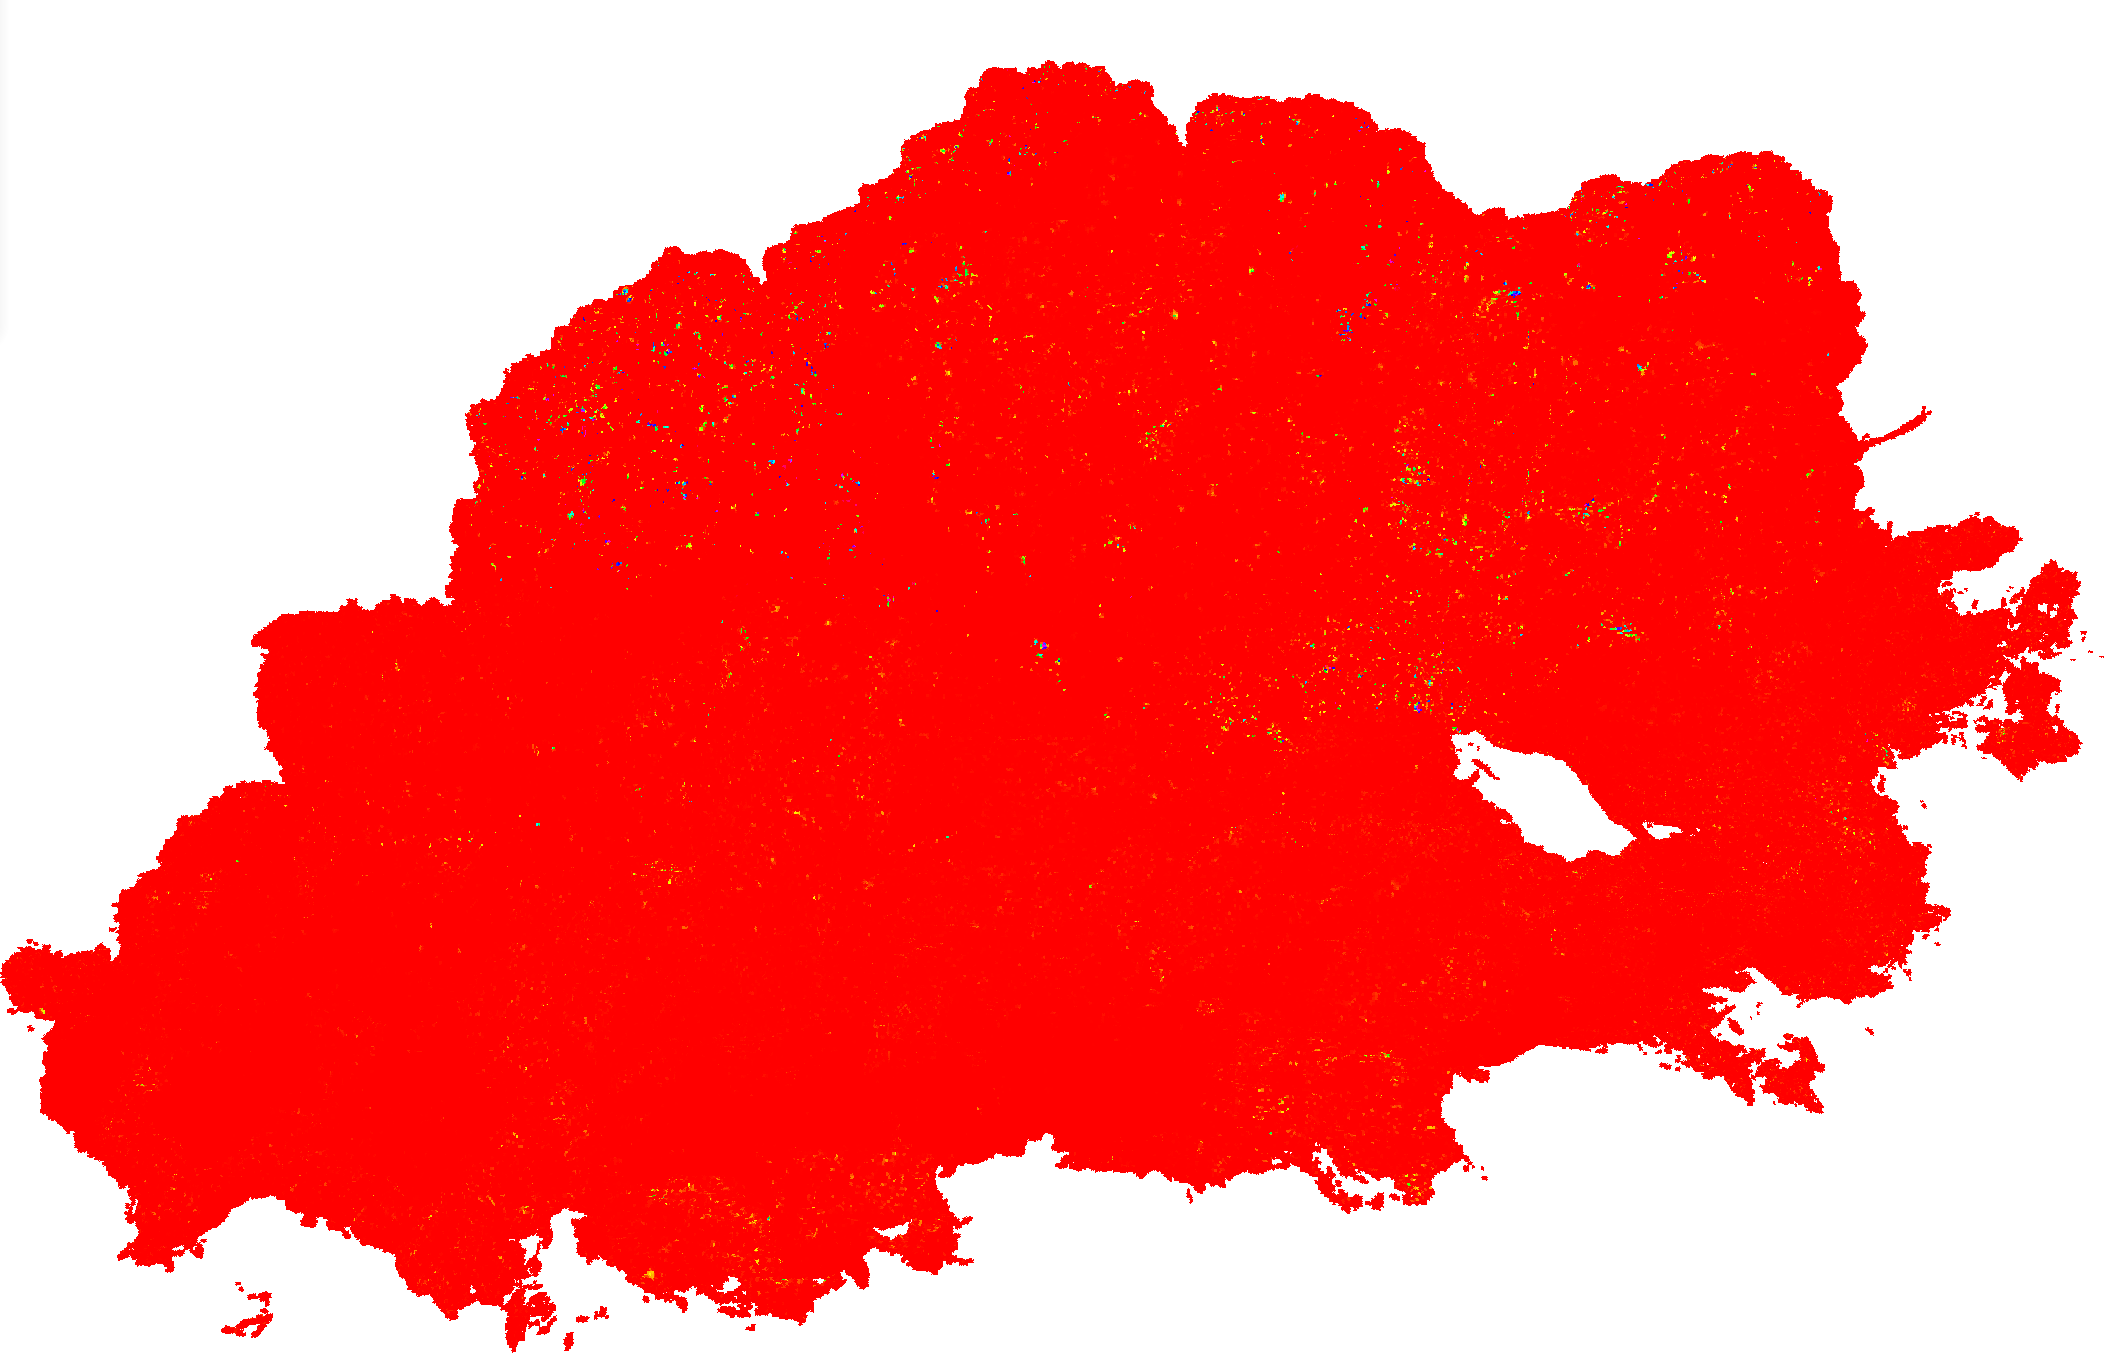
\includegraphics[width=0.45\textwidth]{figures/disney_cloud_half_res_first_temp.png}
    }
    \caption{Some of the shading options of the VDB viewer application. All renders are done using the half resolution version of the Disney cloud \cite{DisneyCloud}. } \label{implementation:vdb_viewer:debug_views}
\end{figure}